\documentclass[11pt,a4paper]{article}

\usepackage[utf8]{inputenc}
\usepackage[T1]{fontenc}
\usepackage[spanish, es-nodecimaldot]{babel}
\addto\captionsspanish{\renewcommand{\tablename}{Tabla}}
\usepackage{geometry}
\geometry{margin=2.5cm}
\usepackage{booktabs}
\usepackage{array}
\usepackage{hyperref}
\hypersetup{colorlinks=true, linkcolor=black, urlcolor=blue}
\usepackage{parskip}
\usepackage{listings}
\usepackage{xcolor}
\usepackage{graphicx}
\graphicspath{{diagrams/}}
\usepackage{float}
\usepackage{caption}
\usepackage{enumitem}

\definecolor{lightgray}{gray}{0.92}
\definecolor{codered}{RGB}{180,30,30}
\definecolor{codegreen}{RGB}{0,120,0}
\definecolor{codegray}{RGB}{100,100,100}
\definecolor{warnorange}{RGB}{200,100,0}

\lstset{
  language=Java,
  basicstyle=\ttfamily\footnotesize,
  keywordstyle=\color{blue}\bfseries,
  commentstyle=\color{codegray}\itshape,
  stringstyle=\color{codegreen},
  showstringspaces=false,
  breaklines=true,
  frame=single,
  framesep=4pt,
  xleftmargin=6pt,
  xrightmargin=6pt,
  aboveskip=6pt,
  belowskip=6pt,
  numbers=left,
  numberstyle=\tiny\color{codegray},
  numbersep=5pt,
}

\newcommand{\code}[1]{\texttt{#1}}
\newcommand{\bad}[1]{\textcolor{codered}{\textbf{#1}}}
\newcommand{\good}[1]{\textcolor{codegreen}{\textbf{#1}}}

\title{Refactorizaci\'on de la clase \code{Variable}\\
       \large Extracci\'on de responsabilidades y consolidaci\'on
              del modelo de dominio\\[4pt]
       \normalsize \code{org.openmarkov.core} --- paquete \code{model.network}}
\author{Manuel Arias Calleja}
\date{Marzo de 2026}

\begin{document}

\maketitle
\tableofcontents
\newpage

% ===================================================================
\section{Introducci\'on}

Este documento describe la refactorizaci\'on de la clase \code{Variable}
del m\'odulo \code{org.openmarkov.core}, que pas\'o de \bad{986~l\'ineas}
a \good{690~l\'ineas} mediante una serie de mejoras incrementales.

La refactorizaci\'on sigue el patr\'on \emph{Extract Class}
\cite{fowler2019} y se fundamenta en el \emph{Principio de
Responsabilidad \'Unica} (SRP) \cite{martin2003}.  Cada concepto se
explica en la secci\'on~\ref{sec:teoria} de forma accesible antes de
describir los cambios concretos.

Todos los cambios se verificaron con una bater\'ia de \textbf{99~tests
unitarios} (71 de ellos nuevos), m\'as los 410~tests del m\'odulo
\code{core}, todos pasando sin errores.

% ===================================================================
\section{Fundamentos te\'oricos}
\label{sec:teoria}

\subsection{Principio de Responsabilidad \'Unica (SRP)}

El \emph{Single Responsibility Principle} establece que \textbf{una clase
debe tener una \'unica raz\'on para cambiar} \cite{martin2003}.  Si una
clase acumula m\'ultiples responsabilidades, un cambio en una de ellas
puede introducir errores en las dem\'as.

\textbf{Ejemplo intuitivo:} pensemos en un documento de texto que
tambi\'en contuviera la l\'ogica de la impresora y del corrector
ortogr\'afico.  Si necesit\'aramos cambiar el formato de impresi\'on,
podr\'iamos romper accidentalmente el corrector.  En software, cada
``responsabilidad'' deber\'ia vivir en su propia clase.

Cuando una clase viola SRP, los s\'intomas t\'ipicos son:

\begin{itemize}
  \item La clase tiene muchas l\'ineas (cientos o miles).
  \item Los m\'etodos se agrupan en bloques tem\'aticos que no se
        relacionan entre s\'i.
  \item Los cambios en una parte de la clase obligan a re-testear partes
        no relacionadas.
  \item Es dif\'icil nombrar la clase con un sustantivo \'unico que
        describa todo lo que hace.
\end{itemize}

\subsection{Patr\'on \emph{Extract Class}}

El patr\'on \emph{Extract Class} \cite{fowler2019} es la t\'ecnica de
refactorizaci\'on que se aplica cuando una clase tiene demasiadas
responsabilidades.  Consiste en:

\begin{enumerate}
  \item Identificar un grupo cohesivo de m\'etodos que forman una
        responsabilidad independiente.
  \item Crear una nueva clase con esos m\'etodos.
  \item En la clase original, sustituir la l\'ogica extra\'ida por una
        \textbf{delegaci\'on} (una llamada a la nueva clase).
\end{enumerate}

En nuestro caso, los m\'etodos extra\'idos no usan campos privados de
\code{Variable} ---solo acceden a m\'etodos p\'ublicos como
\code{getStates()}, \code{setStates()}, \code{getVariableType()}---,
lo que permite moverlos a una \textbf{clase de utilidad est\'atica} que
recibe la \code{Variable} como par\'ametro.

En nuestro caso concreto, los m\'etodos extra\'idos se movieron a una
\textbf{clase de utilidad est\'atica}: una clase no instanciable que
agrupa m\'etodos \code{static} sin estado propio.  Este patr\'on ya se
usa en OpenMarkov; por ejemplo, \code{VariableTypeConverter} fue
extra\'ida previamente de la clase \code{Node} con el mismo enfoque.

\subsection{?`Qu\'e es un acoplamiento?}
\label{sec:acoplamiento}

Decimos que una clase~A est\'a \textbf{acoplada} a otra clase~B cuando
A~necesita conocer la existencia de~B para funcionar.  Un acoplamiento
alto dificulta la reutilizaci\'on y el testing, porque para probar~A hay
que construir tambi\'en~B y todas sus dependencias.

En nuestro caso, \code{Variable} estaba acoplada a \code{Node},
\code{ProbNet}, \code{Link}, \code{Potential} y \code{UniformPotential}
solo por los m\'etodos de edici\'on de estados.  Al extraerlos, la clase
\code{Variable} queda libre de esas dependencias del grafo.

% ===================================================================
\section{Situaci\'on anterior: \code{Variable} con 986~l\'ineas}
\label{sec:antes}

La clase \code{Variable} representaba una variable aleatoria (o de
decisi\'on) en una red bayesiana.  Un diagrama UML simplificado de la
situaci\'on anterior se muestra en la Figura~\ref{fig:antes}.

\begin{figure}[H]
  \centering
  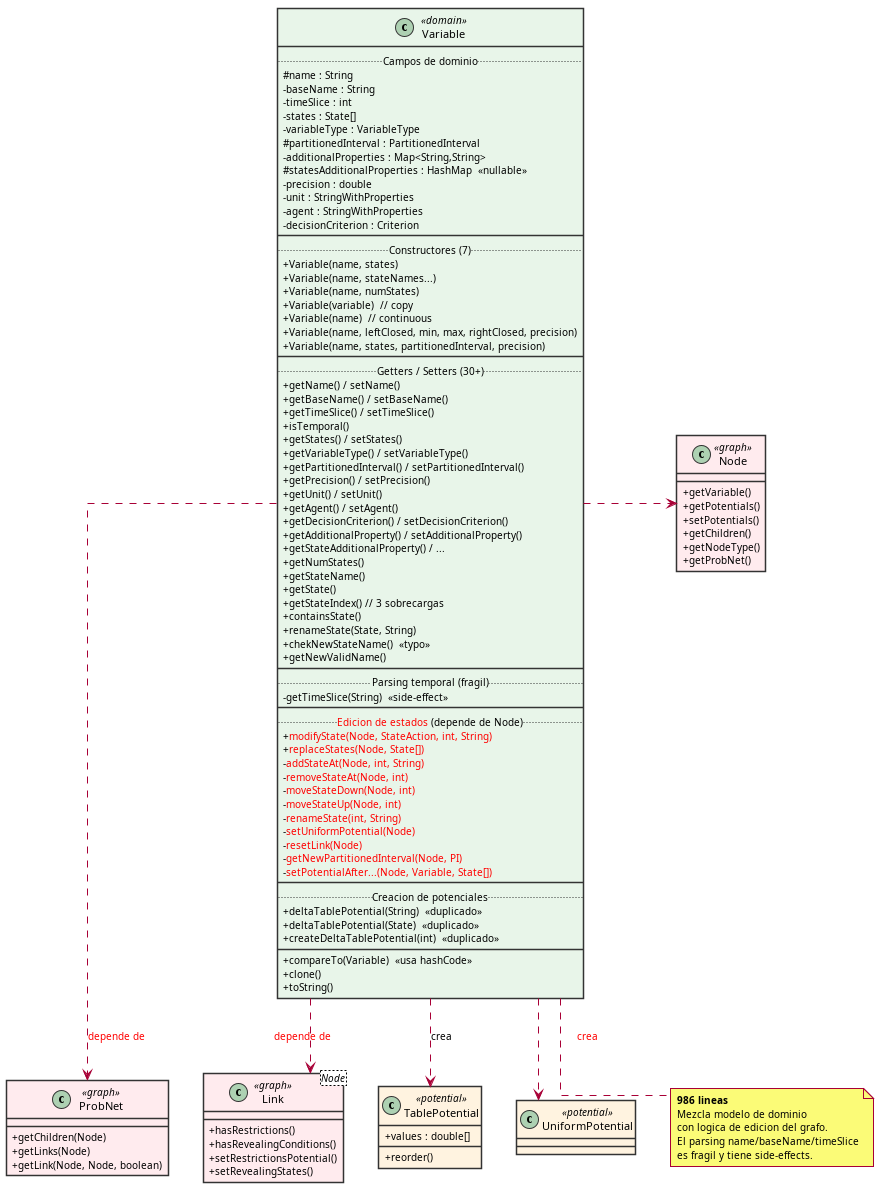
\includegraphics[width=\textwidth]{variable-antes.png}
  \caption{Diagrama UML de \code{Variable} antes de la refactorizaci\'on.
           Los m\'etodos en \textcolor{red}{rojo} son los que depend\'ian
           de \code{Node}/\code{ProbNet}/\code{Link}.}
  \label{fig:antes}
\end{figure}

\subsection{Problemas identificados}

Se identificaron seis problemas principales:

\subsubsection{1. Violaci\'on del SRP: l\'ogica de edici\'on del grafo}
\label{sec:prob-srp}

La clase mezclaba dos responsabilidades claramente distintas:

\begin{itemize}
  \item \textbf{Modelo de dominio}: nombre, tipo, estados, intervalo,
        precisi\'on --- lo que describe a la variable en s\'i misma.
  \item \textbf{Edici\'on del grafo}: m\'etodos como
        \code{addStateAt()}, \code{removeStateAt()},
        \code{setUniformPotential()}, \code{resetLink()} que modifican
        potenciales de nodos hijos, resetean restricciones de arcos,
        etc.
\end{itemize}

Estos \'ultimos m\'etodos recib\'ian un \code{Node} como par\'ametro y
operaban sobre \code{ProbNet}, \code{Link} y diversas subclases de
\code{Potential}.  \textbf{Una variable no deber\'ia conocer la
topolog\'ia del grafo} en el que participa.

En total, \textbf{10~m\'etodos privados y 2~p\'ublicos} (unas
\textbf{180~l\'ineas}) pertenec\'ian a esta responsabilidad ajena.

\subsubsection{2. Inconsistencia name/baseName/timeSlice}
\label{sec:prob-name}

Las variables temporales (como ``X~[3]'') almacenan su nombre en tres
campos interdependientes:

\begin{itemize}
  \item \code{name}: el nombre completo (ej. \code{"X [3]"}).
  \item \code{baseName}: el nombre sin el \'indice temporal (ej. \code{"X"}).
  \item \code{timeSlice}: el \'indice temporal (ej. \code{3}).
\end{itemize}

Exist\'ian \textbf{tres puntos distintos} donde estos campos se
sincronizaban: \code{setName()}, \code{setBaseName()} y
\code{setTimeSlice()}.  Cada uno reimplementaba la l\'ogica de parsing o
reconstrucci\'on de forma ligeramente distinta, y el m\'etodo privado
\code{getTimeSlice(String)} ten\'ia un \emph{side-effect}: modificaba el
campo \code{baseName} como efecto secundario de parsear el nombre.

El propio c\'odigo fuente reconoc\'ia el problema con un TODO:

\begin{lstlisting}
// TODO  mantener la consistencia entre name y baseName cuando se cambian
\end{lstlisting}

\subsubsection{3. Orden de comparaci\'on no determinista}

El m\'etodo \code{compareTo()} comparaba variables por su
\code{hashCode()}, que en Java depende de la direcci\'on de memoria del
objeto.  Esto produce un orden arbitrario que cambia entre ejecuciones
del programa, lo que puede causar comportamientos no reproducibles cuando
las variables se almacenan en colecciones ordenadas.

\subsubsection{4. Inicializaci\'on inconsistente de propiedades}

El campo \code{additionalProperties} se inicializaba como
\code{new HashMap<>()} en la declaraci\'on, pero
\code{statesAdditionalProperties} se dejaba a \code{null}, lo que
obligaba a incluir comprobaciones de nulidad en los cuatro m\'etodos que
lo usaban.

\subsubsection{5. M\'etodo con error tipogr\'afico}

El m\'etodo \code{chekNewStateName()} (falta una ``c'' en \emph{check})
era funcionalmente id\'entico a \code{!containsState()} y no ten\'ia
ning\'un uso en c\'odigo de producci\'on fuera de la propia clase.

\subsubsection{6. Duplicaci\'on en potenciales delta}

Tres m\'etodos ---\code{deltaTablePotential(String)},
\code{deltaTablePotential(State)} y
\code{createDeltaTablePotential(int)}--- conten\'ian l\'ogica duplicada
para crear potenciales delta (distribuciones donde toda la probabilidad
se concentra en un solo estado).

% ===================================================================
\section{Refactorizaci\'on aplicada}
\label{sec:refactorizacion}

La refactorizaci\'on se realiz\'o en seis pasos incrementales, cada uno
verificado con la bater\'ia completa de tests antes de pasar al
siguiente.

\subsection{Paso 1: Ampliaci\'on de tests}

Antes de modificar la clase, se ampli\'o la cobertura de tests de
\textbf{28~tests} a \textbf{99~tests}, a\~nadiendo pruebas para:

\begin{itemize}[nosep]
  \item Todos los constructores (con array de estados, varargs,
        num\'erico, continuo, discretizado, copia).
  \item M\'etodo \code{clone()}.
  \item Propiedades adicionales de variable y de estados.
  \item Variables temporales (parsing, timeSlice, baseName).
  \item Consultas de estados (\code{getState()},
        \code{getStateIndex()}, \code{containsState()}).
  \item Potenciales delta.
  \item Intervalos por defecto y redondeo.
  \item Getters/setters de propiedades (\code{unit}, \code{agent},
        \code{decisionCriterion}).
\end{itemize}

Estos tests actuaron como \textbf{red de seguridad}: si alguna
refactorizaci\'on posterior introduc\'ia una regresi\'on, los tests la
detectar\'ian inmediatamente.

\subsection{Paso 2: Extracci\'on de la l\'ogica de edici\'on de estados
            (\emph{Extract Class})}
\label{sec:extract}

Se cre\'o la clase \code{VariableStateOperations} siguiendo el patr\'on
de \code{VariableTypeConverter} ya existente en el proyecto.

\textbf{M\'etodos extra\'idos} (10~privados + 2~p\'ublicos):

\begin{center}
\footnotesize
\begin{tabular}{ll}
\toprule
\textbf{M\'etodo} & \textbf{Responsabilidad} \\
\midrule
\code{modifyState()} & Dispatcher: ADD, REMOVE, UP, DOWN, RENAME \\
\code{replaceStates()} & Reemplazo completo de estados \\
\code{addStateAt()} & A\~nadir un estado en una posici\'on \\
\code{removeStateAt()} & Eliminar un estado \\
\code{moveStateDown()} & Intercambiar estado con el anterior \\
\code{moveStateUp()} & Intercambiar estado con el siguiente \\
\code{renameState(int, String)} & Renombrar estado por \'indice \\
\code{setUniformPotential()} & Resetear potenciales a distribuci\'on uniforme \\
\code{resetLink()} & Limpiar restricciones de arcos \\
\code{getNewPartitionedInterval()} & Calcular nuevo intervalo tras a\~nadir estado \\
\code{reorderStatesInNodeAndChildren()} & Reordenar potenciales tras mover estado \\
\code{setPotentialAfterReordering...} & Helper de reordenaci\'on \\
\bottomrule
\end{tabular}
\end{center}

En \code{Variable}, los m\'etodos p\'ublicos quedaron como delegaciones
de una l\'inea:

\begin{lstlisting}
public void modifyState(Node node, StateAction action, int idx, String name) {
    VariableStateOperations.modifyState(this, node, action, idx, name);
}
\end{lstlisting}

El flujo de la delegaci\'on se muestra en la
Figura~\ref{fig:delegacion}.

\begin{figure}[H]
  \centering
  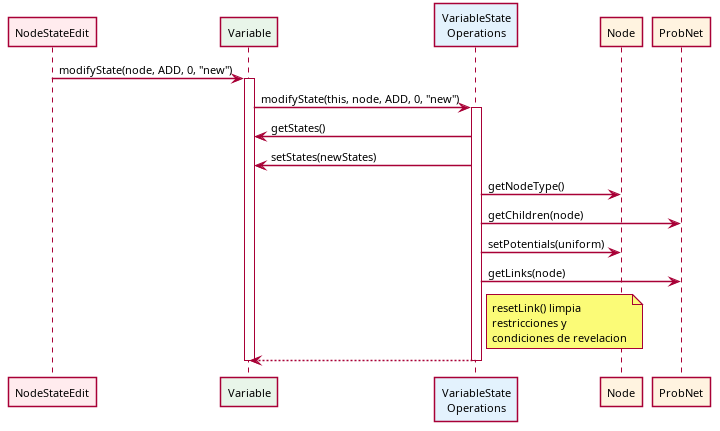
\includegraphics[width=0.85\textwidth]{flujo-delegacion.png}
  \caption{Diagrama de secuencia: flujo de una operaci\'on ADD tras la
           refactorizaci\'on.  \code{Variable} delega a
           \code{VariableStateOperations}, que es quien interact\'ua con
           \code{Node} y \code{ProbNet}.}
  \label{fig:delegacion}
\end{figure}

\subsection{Paso 3: Consolidaci\'on de name/baseName/timeSlice}

Se reemplazaron los tres puntos de sincronizaci\'on por dos m\'etodos
privados:

\begin{itemize}
  \item \code{parseNameIntoParts(String)}: descompone un nombre completo
        como \code{"X [3]"} en \code{baseName="X"} y \code{timeSlice=3}.
        Es el \'unico punto de \emph{parsing}.
  \item \code{rebuildFullName()}: reconstruye \code{name} a partir de
        \code{baseName} y \code{timeSlice}.  Es el \'unico punto de
        \emph{composici\'on}.
\end{itemize}

Todos los constructores y setters usan ahora exclusivamente estos dos
m\'etodos, eliminando el TODO y garantizando la consistencia.  La
Figura~\ref{fig:namesync} muestra la diferencia.

\begin{figure}[H]
  \centering
  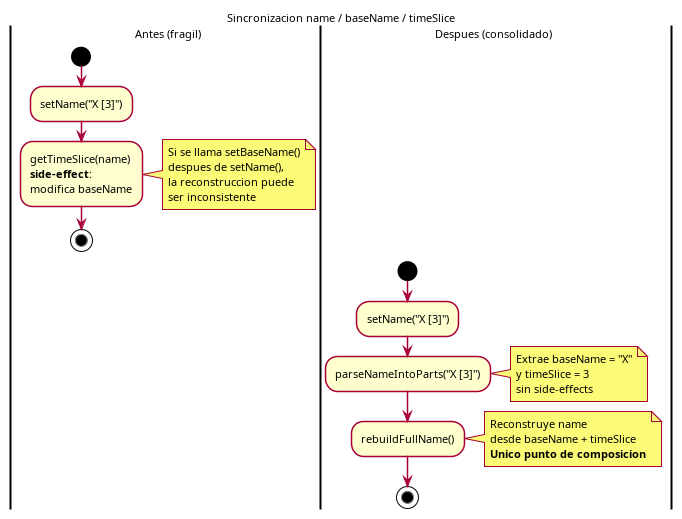
\includegraphics[width=0.75\textwidth]{name-sync.png}
  \caption{Antes y despu\'es de la consolidaci\'on del parsing temporal.
           Antes, \code{getTimeSlice(String)} ten\'ia un side-effect
           sobre \code{baseName}.  Despu\'es, hay un \'unico flujo
           limpio.}
  \label{fig:namesync}
\end{figure}

\subsection{Paso 4: Correcci\'on de \code{compareTo()}}

Se sustituy\'o la comparaci\'on por \code{hashCode()} ---no determinista
entre ejecuciones--- por una comparaci\'on por \code{name} (orden
alfab\'etico):

\begin{lstlisting}
// Antes (no determinista):
@Override public int compareTo(Variable o) {
    int othersHashCode = o.hashCode();
    int thisHashCode = hashCode();
    // ...comparacion por hashCode...
}

// Despues (determinista):
@Override public int compareTo(Variable o) {
    return this.name.compareTo(o.name);
}
\end{lstlisting}

\subsection{Paso 5: Inicializaci\'on \emph{eager} de
            \code{statesAdditionalProperties}}

Se cambi\'o la declaraci\'on del campo de:

\begin{lstlisting}
protected HashMap<...> statesAdditionalProperties;      // null inicial
\end{lstlisting}

a:

\begin{lstlisting}
protected HashMap<...> statesAdditionalProperties = new HashMap<>();
\end{lstlisting}

Esto permiti\'o eliminar las comprobaciones de nulidad en los cuatro
m\'etodos que lo usan y simplificar \code{setStateAdditionalProperty()}
usando \code{computeIfAbsent()}:

\begin{lstlisting}
public void setStateAdditionalProperty(String state, String key, String value) {
    statesAdditionalProperties
            .computeIfAbsent(state, k -> new HashMap<>())
            .put(key, value);
}
\end{lstlisting}

\subsection{Paso 6: Eliminaci\'on de \code{chekNewStateName()} y
            unificaci\'on de potenciales delta}

\begin{itemize}
  \item Se elimin\'o \code{chekNewStateName()} (sin usos en producci\'on,
        equivalente a \code{!containsState()}).
  \item Las tres variantes de \code{deltaTablePotential} se unificaron:
        las versiones con \code{String} y \code{State} ahora delegan en
        \code{createDeltaTablePotential(int)}, eliminando la duplicaci\'on.
\end{itemize}

% ===================================================================
\section{Resultado final}
\label{sec:resultado}

La Figura~\ref{fig:despues} muestra el diagrama UML de la clase
\code{Variable} tras todas las refactorizaciones.

\begin{figure}[H]
  \centering
  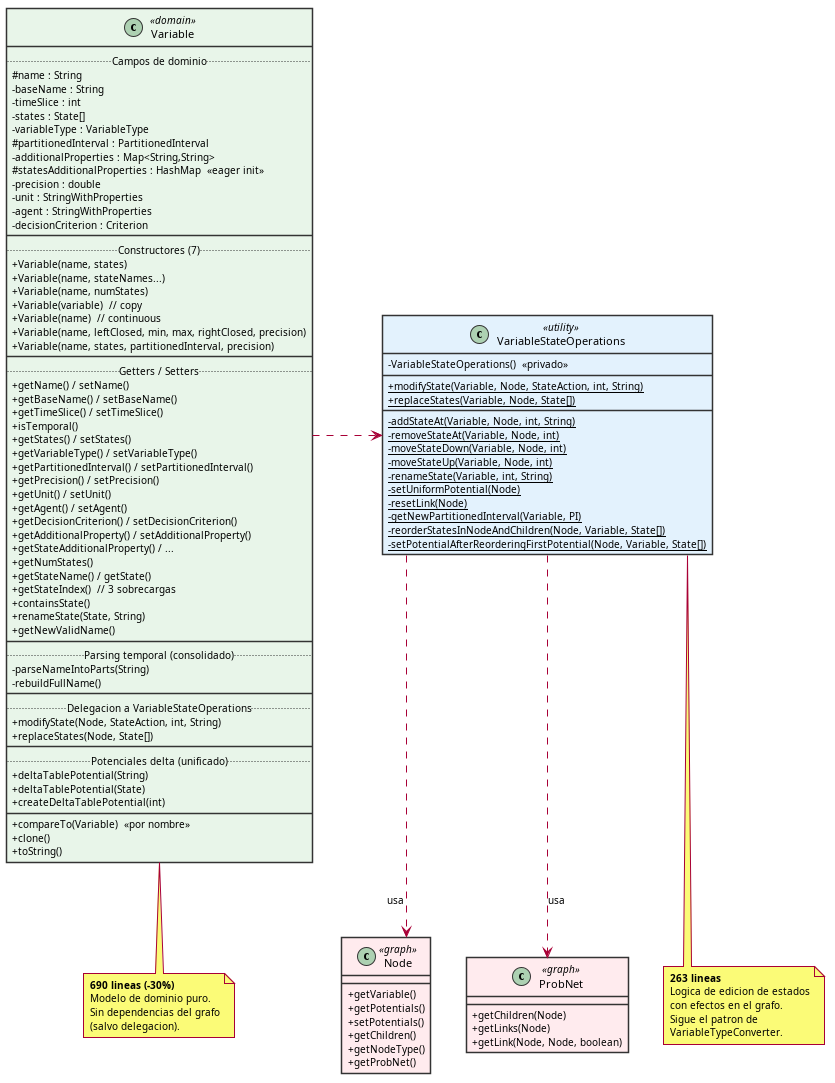
\includegraphics[width=\textwidth]{variable-despues.png}
  \caption{Diagrama UML de \code{Variable} y
           \code{VariableStateOperations} despu\'es de la refactorizaci\'on.
           \code{Variable} es ahora un modelo de dominio puro.}
  \label{fig:despues}
\end{figure}

\subsection{Resumen num\'erico}

\begin{center}
\begin{tabular}{lrr}
\toprule
\textbf{M\'etrica} & \textbf{Antes} & \textbf{Despu\'es} \\
\midrule
L\'ineas de \code{Variable.java} & 986 & \good{690 (--30\%)} \\
Dependencias de \code{Variable} hacia el grafo & 4 clases & \good{0 (delegaci\'on)} \\
M\'etodos p\'ublicos duplicados & 3 & \good{0} \\
Null checks en \code{statesAdditionalProperties} & 5 & \good{0} \\
Puntos de sincronizaci\'on name/baseName & 3 & \good{2 (centralizados)} \\
Tests unitarios & 28 & \good{99} \\
Tests del m\'odulo core & 410 & 408\footnotemark \\
Tests fallidos & 0 & \good{0} \\
\bottomrule
\end{tabular}
\end{center}

\footnotetext{La diferencia de 2~tests se debe a la eliminaci\'on de
los tests del m\'etodo \code{chekNewStateName()}, que fue eliminado.}

\subsection{Ficheros afectados}

\begin{center}
\footnotesize
\begin{tabular}{lp{8cm}}
\toprule
\textbf{Fichero} & \textbf{Cambio} \\
\midrule
\code{Variable.java} & Eliminados 10 m\'etodos privados, consolidado
  parsing, simplificados null checks, eliminado m\'etodo con typo,
  corregido \code{compareTo()}, unificados delta potentials \\
\code{VariableStateOperations.java} & \textbf{Nuevo} (263~l\'ineas) ---
  l\'ogica de edici\'on de estados extra\'ida de \code{Variable} \\
\code{VariableTest.java} & Ampliado de 4 a 47~tests (m\'as nested classes) \\
\code{VariableModifyStateTest.java} & Sin cambios (24~tests siguen pasando) \\
\code{NodeStateEdit.java} & Sin cambios \\
\code{NodeReplaceStatesEdit.java} & Sin cambios \\
\bottomrule
\end{tabular}
\end{center}

% ===================================================================
\section{Verificaci\'on}
\label{sec:verificacion}

Cada paso de la refactorizaci\'on se verific\'o ejecutando:

\begin{lstlisting}[language=bash, numbers=none]
# Tests especificos de Variable
mvn test -pl org.openmarkov.core \
    -Dtest="VariableTest,VariableModifyStateTest"

# Todos los tests del modulo core
mvn test -pl org.openmarkov.core
\end{lstlisting}

En todos los pasos, los 408~tests del m\'odulo \code{core} pasaron con
0~fallos y 0~errores.

% ===================================================================
\section{Conclusiones}

La refactorizaci\'on de \code{Variable} logr\'o:

\begin{enumerate}
  \item \textbf{Separar responsabilidades}: la l\'ogica de edici\'on del
        grafo ahora reside en \code{VariableStateOperations}, y
        \code{Variable} es un modelo de dominio puro.
  \item \textbf{Eliminar fragilidad}: la sincronizaci\'on
        name/baseName/timeSlice se centraliz\'o en dos m\'etodos,
        eliminando el riesgo de inconsistencias.
  \item \textbf{Mejorar la mantenibilidad}: c\'odigo m\'as corto, sin
        null checks innecesarios, sin duplicaciones, y con un orden de
        comparaci\'on determinista.
  \item \textbf{Aumentar la confianza}: la bater\'ia de tests se
        multiplic\'o por~3,5, cubriendo \'areas que antes no se probaban.
  \item \textbf{Mantener compatibilidad}: no se modific\'o ninguna clase
        llamadora (\code{NodeStateEdit}, \code{NodeReplaceStatesEdit}),
        gracias al patr\'on de delegaci\'on.
\end{enumerate}

La refactorizaci\'on sigue el precedente establecido por la extracci\'on
previa de \code{VariableTypeConverter} desde \code{Node}, manteniendo la
coherencia arquitect\'onica del proyecto.

% ===================================================================
\begin{thebibliography}{9}

\bibitem{fowler2019}
  M. Fowler,
  \emph{Refactoring: Improving the Design of Existing Code},
  2nd ed., Addison-Wesley, 2019.

\bibitem{martin2003}
  R.C. Martin,
  \emph{Agile Software Development: Principles, Patterns, and Practices},
  Prentice Hall, 2003.

\end{thebibliography}

\end{document}
